%%%%%%%%%%%%%%%%%%%%%%%%%%%%%%%%%%%%%%%%%%%%%%%%%%%%%%%%%%%%%%%%%%%%%%%%%
% ARTICLE ABOUT FATE OF SYNONYMOUS MUTATIONS IN HIV
%%%%%%%%%%%%%%%%%%%%%%%%%%%%%%%%%%%%%%%%%%%%%%%%%%%%%%%%%%%%%%%%%%%%%%%%%
\documentclass[rmp, twocolumn]{revtex4}
%%%%%%%%%%%%%%%%%%%%%%%%%%%%%%%%%%%%%%%%%%%%%%%%%%%%%%%%%%%%%%%%%%%%%%%%%
%%%%%%%%%%%%%%%%%%%%%%%%%%%%%%%%%%%%%%%%%%%%%%%%%%%%%%%%%%%%%%%%%%%%%%%%%
\usepackage[english]{babel}
\usepackage[utf8x]{inputenc}
\usepackage{amsmath,amsfonts,amssymb,eucal,eurosym,textcomp}
\usepackage{color}
\usepackage{graphicx}
\usepackage[caption=false]{subfig}
\usepackage{natbib}
\usepackage{pslatex}
%%%%%%%%%%%%%%%%%%%%%%%%%%%%%%%%%%%%%%%%%%%%%%%%%%%%%%%%%%%%%%%%%%%%%%%%%
\graphicspath{{./figures/}}
%%%%%%%%%%%%%%%%%%%%%%%%%%%%%%%%%%%%%%%%%%%%%%%%%%%%%%%%%%%%%%%%%%%%%%%%%
\newcommand{\comment}[1]{\textit{\textcolor{red}{#1}}}
\newcommand{\mut}{\mu}
\newcommand{\mfit}{\langle F\rangle}
\newcommand{\mexpfit}{\langle e^{F}\rangle}
\newcommand{\pfix}{P_{\mathrm{fix}}}
\newcommand{\ox}{r}
\newcommand{\co}{\rho}
\newcommand{\gt}{g}
\newcommand{\locus}{s}
\newcommand{\locuspm}{t}
\newcommand{\OO}{\mathcal{O}}
\newcommand{\rev}{\textit{rev}}
\newcommand{\FIG}[1]{Fig.~\ref{fig:#1}}
\newcommand{\FIGS}[2]{Figs.~\ref{fig:#1} and~\ref{fig:#2}}
\newcommand{\env}{\textit{env}}
\newcommand{\shankaregion}{C2-V5}
\newcommand{\PCApat}{1}
\newcommand{\syndiv}{2}
\newcommand{\timedependence}{3}
\newcommand{\withinepi}{4}
%%%%%%%%%%%%%%%%%%%%%%%%%%%%%%%%%%%%%%%%%%%%%%%%%%%%%%%%%%%%%%%%%%%%%%%%%
\renewcommand{\thesubfigure}{\Alph{subfigure}}
\newcommand{\Author}{Fabio~Zanini and Richard~A.~Neher}
\newcommand{\Title}{Quantifying selection against synonymous mutations in HIV-1 \env{} evolution}
\newcommand{\Affiliation}{Max Planck Institute for Developmental Biology, 72076 T\"ubingen, Germany}
\newcommand{\Keywords}{{HIV}, {synonymous}, {population genetics}}
%%%%%%%%%%%%%%%%%%%%%%%%%%%%%%%%%%%%%%%%%%%%%%%%%%%%%%%%%%%%%%%%%%%%%%%%%
\usepackage{hyperref}
\hypersetup{colorlinks,linkcolor=red,citecolor=blue, pdfauthor={\Author}, pdftitle={\Title}, pdfkeywords={\Keywords}}
%%%%%%%%%%%%%%%%%%%%%%%%%%%%%%%%%%%%%%%%%%%%%%%%%%%%%%%%%%%%%%%%%%%%%%%%%
\begin{document}
\title{\Title}
\author{\Author}
\affiliation{\Affiliation}
\date{\today}
%%%%%%%%%%%%%%%%%%%%%%%%%%%%%%%%%%%%%%%%%%%%%%%%%%%%%%%%%%%%%%%%%%%%%%%%%

\begin{abstract}
\noindent
Intrapatient HIV-1 evolution is dominated by selection on the protein level in
the arms race with the adaptive immune system. When cytotoxic CD8${}^+$ T-cells
or neutralizing antibodies target a new epitope, the virus often escapes via
nonsynonymous mutations that impair recognition. Synonymous mutations do not
affect this interplay and are often assumed to be neutral. We analyze
longitudinal intrapatient data from the \shankaregion{} part of the envelope
gene (\env{}) and observe that synonymous mutations rarely spread even though
they often reach high frequencies in the viral population. Using published data
from the SHAPE assay, we find that synonymous mutations that disrupt base pairs
in RNA stems flanking the V loops of gp120 are more likely to be lost than other
synonymous changes, suggesting a function of these RNA hairpins in HIV-1.
Computational modeling indicates that these synonymous mutations have a
selection coefficient of the order of $-0.002$ and that they are brought up to
high frequency by genetic hitchhiking on neighboring beneficial variants. We
conclude that, contrary to common assumptions, synonymous mutations in the V
loops region are neither independent of the escape patterns nor neutral; further
studies are needed to clarify the function of the RNA hairpins found there.
\end{abstract}
%%%%%%%%%%%%%%%%%%%%%%%%%%%%%%%%%%%%%%%%%%%%%%%%%%%%%%%%%%%%%%%%%%%%%%%%%
\maketitle
%%%%%%%%%%%%%%%%%%%%%%%%%%%%%%%%%%%%%%%%%%%%%%%%%%%%%%%%%%%%%%%%%%%%%%%%%
\section{Introduction}
%%%%%%%%%%%%%%%%%%%%%%%%%%%%%%%%%%%%%%%%%%%%%%%%%%%%%%%%%%%%%%%%%%%%%%%%%
HIV-1 evolves rapidly within a single host during the course of the infection.
This evolution is driven by strong selection imposed by the host immune system
via cytotoxic CD8${}^+$ T-cells (CTLs) and neutralizing antibodies
(nAbs)~\citep{rambaut_causes_2004} and facilitated by the high mutation rate
~\citep{mansky_lower_1995,abram_nature_2010}. When the host develops a CTL or
nAb response against a particular HIV-1 epitope, mutations in the viral genome that
reduce or prevent recognition of the epitope frequently emerge. Escape mutations
in epitopes targeted by CTLs typically emerge during early infection and spread
rapidly through the population~\citep{mcmichael_immune_2009}. During chronic
infection, the most rapidly evolving parts of the HIV-1 genome are the variable
loops V1-V5 in the envelope protein gp120, which change to avoid recognition by
nAbs. Escape mutations in \env, the gene encoding gp120, spread through the
viral population within a few months.
Consistent with this time scale, it is found that serum from a particular time
typically neutralizes virus extracted more than 3-6 months earlier but not contemporary
virus \citep{richman_rapid_2003}.

Escape mutations are selected because they change the amino acid sequence of
viral proteins in a way that reduces antibody binding or epitope presentation.
Conversely, synonymous mutations do not modify the viral protein and are
commonly used as approximately neutral markers in studies of viral evolution.
Neutral markers are very useful as a negative control for detecting selected
sites \citep{Bhatt:2011p43255,Hurst:2002p32608,Chen:2004p22606}. In addition to
maintaining protein function and avoiding the adaptive immune recognition,
however, the HIV-1 genome has to ensure efficient processing and translation,
nuclear export, and packaging into the viral capsid: all these processes operate
at the RNA level and are sensitive to synonymous changes. For example, the HIV-1
\rev{} response element (RRE) in \env{} enhances nuclear export of full length
or partially spliced viral transcripts via a complex hairpin RNA structure
\citep{fernandes_hiv-1_2012}. Another well studied case is the interaction
between viral reverse transcriptase, viral ssRNA, and the host
tRNA$^\text{Lys3}$: the latter is required for priming reverse transcription
(RT) and is bound by a pseudoknotted RNA structure in the viral 5' untranslated
region~\citep{barat_interaction_1991, paillart_vitro_2002}. These RNA
structures, but not the exact base pairs, are well conserved between HIV-1 and
SIV \citep{pollom_comparison_2013}.

Even in the absence of important RNA structures, synonymous codons do not evolve
completely neutrally. Some codons are favored in many species
\citep{plotkin_synonymous_2011}. Recent studies have shown that genetically
engineered HIV-1 strains with altered codon usage show differences in gene
expression and replication capacity \citep{ngumbela_quantitative_2008,
li_codon-usage-based_2012, keating_rich_2009}. Codon deoptimization has been
suggested as an attenuation strategy for polio and
influenza~\citep{mueller_live_2010,coleman_virus_2008}. Purifying selection
beyond the protein sequence is therefore expected
\citep{forsdyke_reciprocal_1995,snoeck_mapping_2011}, and it has been shown that
rates of evolution at synonymous sites vary along the HIV-1 genome
\citep{mayrose_towards_2007} (see also \figurename~S\syndiv). Positive
selection through the host adaptive immune system, however, is restricted to
changes in the amino acid sequence.

In this paper, we characterize the dynamics of synonymous mutations in \env{}
and show that, in the region of the V loops, a large fraction of these mutations
is deleterious. Contrary to common assumptions, deleterious synonymous mutations
rise in frequency in the viral population via genetic hitchhiking due to limited
recombination in HIV-1 populations~\citep{neher_recombination_2010,
batorsky_estimate_2011}. We show a strong correlation between the fate of a
synonymous mutation and the surrounding RNA structure, suggesting an important
role of RNA hairpins around V-loops in HIV-1 evolution. We then compare our
observations to computational models and derive estimates for the effect of
synonymous mutations on viral fitness. Extending the analysis of fixation
probabilities to the nonsynonymous mutations, we show that time-dependent
selection or strong competition of escape mutations inside the same epitope are
necessary to explain the observed patterns of fixation and loss.

%%%%%%%%%%%%%%%%%%%%%%%%%%%%%%%%%%%%%%%%%%%%%%%%%%%%%%%%%%%%%%%%%%%%%%%%%
\section{Results}
%%%%%%%%%%%%%%%%%%%%%%%%%%%%%%%%%%%%%%%%%%%%%%%%%%%%%%%%%%%%%%%%%%%%%%%%%
In HIV-1, because of the high mutation rate, single nucleotide variants (SNVs)
are continuously injected into the viral population. We say that an SNV has a
frequency $\nu$ at a certain time if it is found in a fraction $\nu$, between
zero and one, of the sequences from that time point. An SNV rises or falls in
frequency by virtue of both (i) its own effect on fitness and escape and (ii)
the effect of its genetic background. When an SNVs is present in all sequences
at a certain time point, we say it has ``fixed''; when it is completely absent,
we say it was ``lost'' or is ``extinct''. Eventually, all SNVs will fix or be lost; the
probability of fixation is higher for beneficial SNVs, and lower for deleterious
ones. The intermediate case are neutral SNVs: a neutral mutation segregating at
frequency $\nu$ has a probability $\pfix(\nu) = \nu$ to spread through the
population and fix; in the rest of the cases it goes extinct. For instance, if
a neutral SNV is observed in half of the sequences, it will fix with a probability of
50\% (see inset in figure \ref{fig:aftsyn}).

The problem with the classification based on beneficial/neutral/deleterious is
that, given an SNV, we do not know its class \textit{a priori}. Synonymous SNVs,
however, are usually assumed to be neutral. \FIG{aft} shows the time course of
the frequencies of all synonymous and nonsynonymous viral mutations observed in
\env, in \shankaregion, in a chronically HIV-1 infected patient (p10
from \citet{shankarappa_consistent_1999}). Despite many synonymous SNVs
reaching high frequency, very few fix (panel~\ref{fig:aftsyn}); in constrast, many
nonsynonymous mutations fix (panel~\ref{fig:aftnonsyn}). This basic observation
seems at odds with the assumption of neutrality.

%%%%%%%%%%%%%%%%%%%%%%%%%%%%%%%%%%%%%%%%%%%%%%%%%%%%%%%%%%%%%%%%%%%%%%%%%
\subsection{Many synonymous polymorphisms in \shankaregion{} are deleterious}
%%%%%%%%%%%%%%%%%%%%%%%%%%%%%%%%%%%%%%%%%%%%%%%%%%%%%%%%%%%%%%%%%%%%%%%%%
We study the dynamics and fate of synonymous SNVs more quantitatively by
analyzing data from seven patients from \citet{shankarappa_consistent_1999} and
\citep{liu_selection_2006} as well as three patients from
\citet{bunnik_autologous_2008} (patients with strong viral population structure
were excluded from the analysis; see methods and \figurename~S\PCApat). The
former data set is restricted to the \shankaregion{} region of \env, while the
data from \citet{bunnik_autologous_2008} cover most of \env.  We consider all
SNVs in a frequency interval $[\nu_0-\delta\nu, \nu_0+\delta\nu]$ at some time
$t$, and calculate the fraction that are still observed at later times $t+\Delta
t$. Plotting this fraction against the time interval $\Delta t$, we see that
most synonymous SNVs segregate for roughly one year and are lost much more
frequently than expected under neutrality (panel \ref{fig:fixp1}). The long-time
probability of fixation, $\pfix$, is shown as a function of the initial
frequency $\nu_0$ in panel \ref{fig:fixp2}. We find that $\pfix$ of synonymous
variants is far below the neutral expectation in \shankaregion (red line).
Outside of \shankaregion, using data from \citet{bunnik_autologous_2008} only,
we find no such reduction in $\pfix$ (green line). Restricted to the
\shankaregion{} region, the sequence samples from \citet{bunnik_autologous_2008}
are fully compatible with data from \citet{shankarappa_consistent_1999}. The
nonsynonymous SNVs seem to follow more or less the neutral expectation (blue
line) -- a point to which we will come back below.

\begin{figure}
\begin{center}
\subfloat{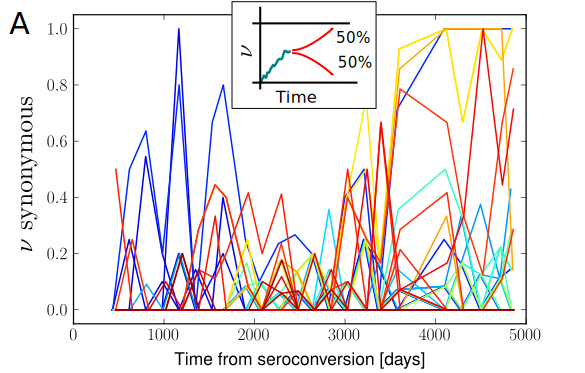
\includegraphics[width=\linewidth]
{Shankarappa_allele_freqs_trajectories_syn_p10.pdf}
\label{fig:aftsyn}}\\
 \subfloat{\includegraphics[width=\linewidth]
{Shankarappa_allele_freqs_trajectories_nonsyn_p10.pdf}
\label{fig:aftnonsyn}}
\caption{Time series of frequencies
of synonymous (A) and nonsynonymous (B) single nucleotide variants (SNVs) in \env, 
\shankaregion, from patient p10~\cite{shankarappa_consistent_1999}.
While many nonsynonymous SNVs fix, few synonymous
SNVs do so even though they are frequently observed at high
frequencies. Colors indicate the position of the site along the \shankaregion{} region
(blue to red). Inset: the fixation probability $\pfix$ of a neutral
SNV that reached 50\% frequency is one half.}
\label{fig:aft}
\end{center}
\end{figure}

When interpreting these results for the fixation probabilities, it is important
to note that we focus on SNVs that have already reached high frequencies. In
HIV-1 infection, most SNVs remain very rare throughout; they are not considered
here. Synonymous SNVs can reach high frequencies by two means, either genetic
drift or genetic hitchhiking on escape variants (see below); very deleterious
variants will never reach high frequencies in the first place. Hence, our
analysis indicates that, among all synonymous SNVs that somehow reach high
frequencies, most of them are deleterious in \shankaregion{}, while they tend to
be neutral in the rest of \env{}.

\begin{figure}
\begin{center}
\subfloat{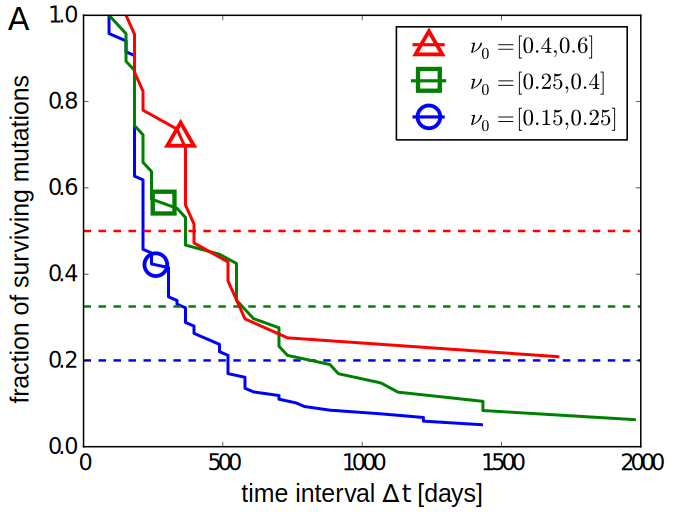
\includegraphics[width=0.9\linewidth]{fixation_times.pdf}
\label{fig:fixp1}}\\
\subfloat{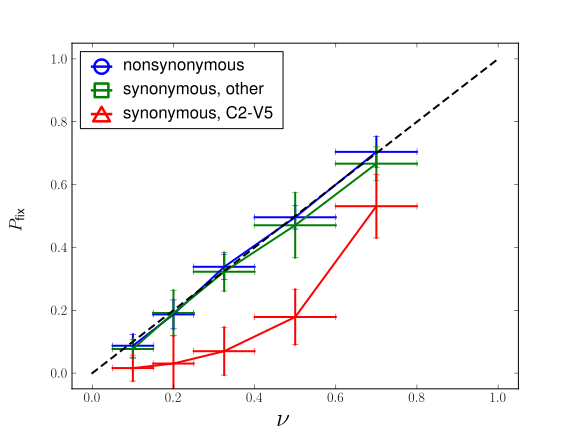
\includegraphics[width=0.9\linewidth]{fixation_probabilities.pdf}
\label{fig:fixp2}}
\caption{Fixation and loss of SNVs.
Panel A) shows how quickly synonymous SNVs are purged from the populations. 
Specifically, the figure shows the fraction of SNVs that are still observed
after $\Delta t$ days, conditional on being observed in one of the three frequency 
intervals (different colors). 
In each frequency interval, the fraction of synonymous
SNVs that ultimately survive is the fixation probability $\pfix$ conditional on the
initial frequency. The neutral expectation for $\pfix=\nu_0$ is indicated by 
dashed horizontal lines.
Panel B) shows the fixation probability of synonymous SNVs as a function of $\nu_0$. Polymorphisms within \shankaregion{} fix less
often than expected for neutral SNVs (indicated by the diagonal line).
This suppression is not observed in other parts of \env{} or for nonsynonymous
SNVs.
The horizontal error bars on the abscissa are bin sizes, the vertical ones the
standard deviation after 100 patient bootstraps of the data. Data from
refs.~\cite{shankarappa_consistent_1999,liu_selection_2006, bunnik_autologous_2008}.}
\label{fig:fixp}
\end{center}
\end{figure}

%%%%%%%%%%%%%%%%%%%%%%%%%%%%%%%%%%%%%%%%%%%%%%%%%%%%%%%%%%%%%%%%%%%%%%%%%
\subsection{Synonymous mutations in \shankaregion{} tend to disrupt RNA stems}
%%%%%%%%%%%%%%%%%%%%%%%%%%%%%%%%%%%%%%%%%%%%%%%%%%%%%%%%%%%%%%%%%%%%%%%%%
One possible explanation for lack of fixation of synonymous SNVs in
\shankaregion{} is secondary structures in the viral RNA, the disruption of which
is deleterious to the virus \citep{forsdyke_reciprocal_1995,
snoeck_mapping_2011, sanjuan_interplay_2011}.

The propensity of nucleotides in the HIV-1 genome to form base pairs has been
measured using the SHAPE assay, a biochemical reaction preferentially altering
unpaired bases (the HIV-1 genome is a single stranded RNA)
\citep{watts_architecture_2009}. The SHAPE assay has shown that the variable
regions V1-V5 tend to be unpaired, while the conserved regions between those
variable regions form stems. We aligned the within-patient sequence samples to
the reference NL4-3 strain used in \citet{watts_architecture_2009} and assigned
SHAPE reactivities to most positions in the alignment. We then calculated the
distributions of SHAPE reactivities for synonymous SNVs that fixed or were
subsequently lost (only SNVs with frequencies above 15\%). As shown in
\FIG{SHAPEA}, the reactivities of fixed SNVs (red histogram) are systematically
larger than those of lost SNVs (blue) (Kolmogorov-Smirnov test on the cumulative
distribution, $p\approx 0.002$). In other words, SNVs that are likely to
break RNA helices are also more likely to revert and finally be lost from the
population, restoring the helix. Note that this analysis will be sensitive only
at positions where the base pairing pattern of NL4-3 agrees with that of each
patient's initial consensus sequence -- it is thus statistically conservative.
As a control, we also calculate the distribution of SHAPE reactivities for SNVs
that never reach high frequencies (green). This set is a mixture of neutral and
deleterious SNVs and, as expected, their distribution lies between those of
fixed and lost high-frequency SNVs.

To test the hypothesis that synonymous SNVs in \shankaregion{} are lost because they
break stems in the conserved stretches between the V loops, we consider
separately SNVs in V loops and conserved flanks. The greatest
depression in fixation probability is observed in the conserved stems, while the
V loops show little deviation from the neutral signature, see
\FIG{SHAPEB}. This is suggestive of important RNA helices in conserved
regions between the V loops.

In addition to RNA secondary structure, we have considered other possible
explanations for a fitness cost of some synonymous mutations, in particular
codon usage bias (CUB). HIV-1 is known to prefer A-rich codons over highly
expressed human codons \citep{jenkins_extent_2003, kuyl_biased_2012}. We do not
find, however, any evidence for a contribution of average CUB to the ultimate
fate of synonymous SNVs; this agrees with the observation that HIV-1 is not
adapting its codon usage to its human host cells at the macroevolutionary level
\citep{kuyl_biased_2012}.

\begin{figure}
\begin{center}
\subfloat{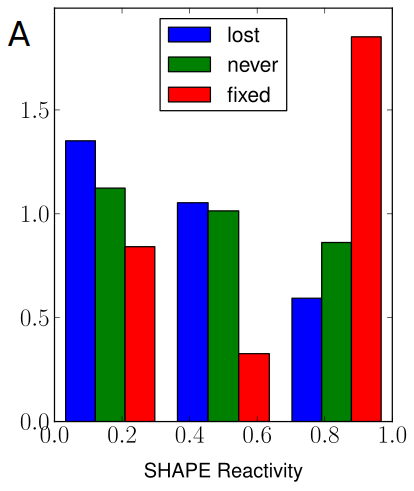
\includegraphics[height=0.50\linewidth]{reactivities_histograms_syn.pdf}\label{fig:SHAPEA}}
\subfloat{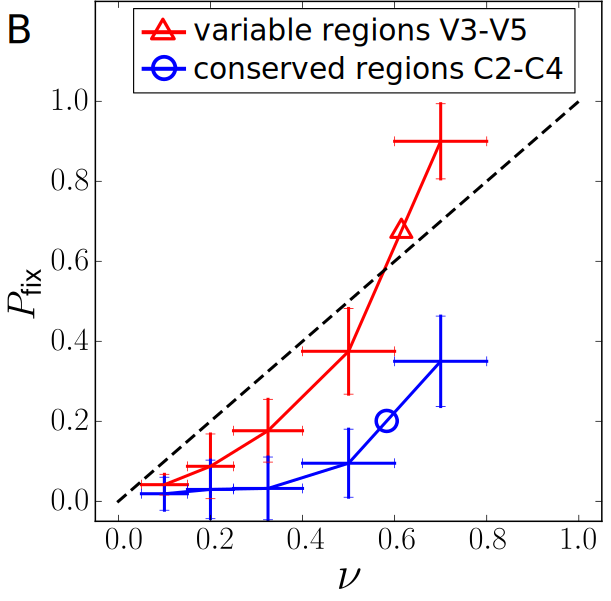
\includegraphics[height=0.49\linewidth]{fixation_probabilities_VnonV.pdf}\label{fig:SHAPEB}}
\caption{Permissible synonymous mutations tend to be unpaired.
Panel A) shows the distribution of SHAPE reactivities among sites at which synonymous 
SNVs fixed (red), sites at which SNVs reached frequencies above 15\% but
were susequently lost (blue), and sites at which no high-frequency SNVs were observed (green) 
(all categories are restricted to the regions V1-V5$\pm 100$bp).
Sites at which SNVs fixed tend to have higher SHAPE reactivities, corresponding to
less base pairing, than those at which SNVs are lost.
Sites at which no SNVs are observed show an intermediate distribution of SHAPE values.
Panel B) shows the fixation probability of synonymous SNVs in
\shankaregion{} separately for variable regions V3-V5 and the connecting conserved 
regions C2-C4 that harbor RNA stems. As expected, the fixation probability is lower
inside the conserved regions. Data from Refs.~\cite{shankarappa_consistent_1999,
bunnik_autologous_2008, liu_selection_2006}.}
\label{fig:SHAPE}
\end{center}
\end{figure}

%%%%%%%%%%%%%%%%%%%%%%%%%%%%%%%%%%%%%%%%%%%%%%%%%%%%%%%%%%%%%%%%%%%%%%%%%
\subsection{Deleterious SNVs reach high frequency by hitchhiking}
%%%%%%%%%%%%%%%%%%%%%%%%%%%%%%%%%%%%%%%%%%%%%%%%%%%%%%%%%%%%%%%%%%%%%%%%%

While the observation that some fraction of synonymous SNVs is deleterious
is not unexpected, it seems odd that we observe them at high population
frequency and that the fixation probability is reduced only in parts of the
genome (in \shankaregion{} but not in the rest of \env{}; compare the red
triangle line versus the green square line in \FIG{fixp2}).
The region \shankaregion{} undergoes frequent adaptive changes to evade
recognition by neutralizing antibodies \cite{williamson_adaptation_2003,
richman_rapid_2003}. Due to the limited amount of recombination in HIV-1
\cite{neher_recombination_2010, batorsky_estimate_2011}, deleterious SNVs
that are linked to adaptive variants can reach high frequency. This process is
known as hitchhiking \citep{smith_hitch-hiking_1974} or genetic draft
\citep{gillespie_genetic_2000,neher_genetic_2011}. Hitchhiking is apparent in
\FIG{aft}, which shows that many SNVs change rapidly in frequency as a
flock. 

The approximate magnitude of the deleterious effects can be estimated from
\FIG{fixp1}, which shows the distribution of times after which synonymous
SNVs at intermediate frequencies become fixed or lost. The typical time to
loss is of the order of 500 days. If this loss is driven by the deleterious
effect of the mutation, this corresponds to deleterious effects $s_d$ of the
order of $- 0.002$ per day. (This is only an average estimate: every single
mutation is expected to have a slightly different fitness effect.)

\begin{figure}
\begin{center}
\subfloat{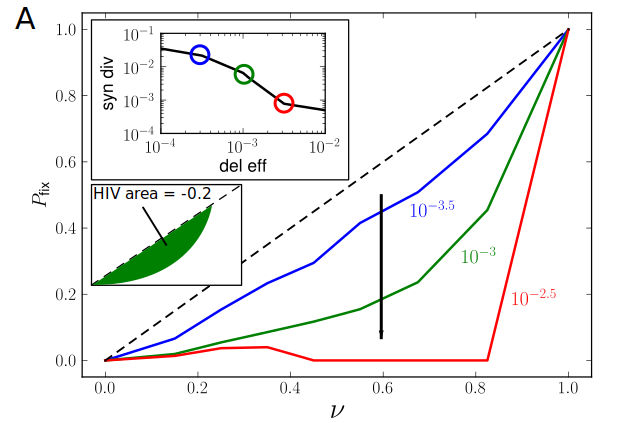
\includegraphics[width=0.9\linewidth]{simulations_graduallydel.pdf}
\label{fig:simfixpvar}}\\
\subfloat{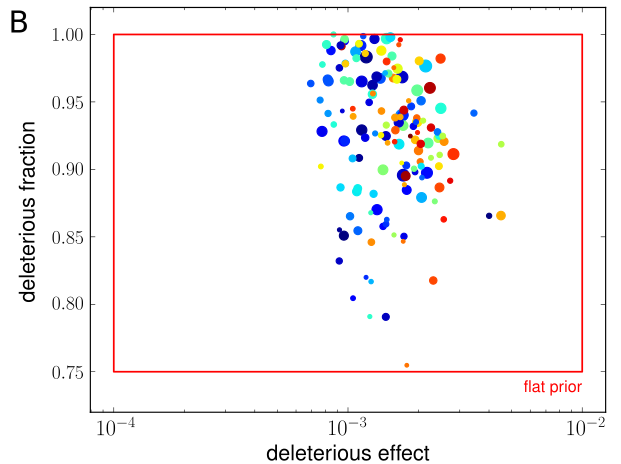
\includegraphics[width=0.9\linewidth]{simulations_syn.pdf}
\label{fig:simsfig}}
\caption{Distribution of selection coefficients on synonymous sites. Panel A)
The depression in $\pfix$ depends on the deleterious effect size 
of synonymous SNVs. This parameter also reduces synonymous
diversity, measured by the probability of a SNV to be found at
intermediate frequencies $P_\text{interm}$ (first inset).
Panel B) To assess the parameter space that affects synonymous fixation and
diversity, we run 2400 simulations with random parameters for deleterious effect
size, fraction of deleterious synonymous sites, average escape rate $\epsilon$
(color, blue to red corresponds to $10^{-2.5}$ to $10^{-1.5}$ per day), and rate of
introduction of new epitopes (marker size, from $10^{-3}$ to $10^{-2}$ per
day). Only simulations that reproduce the synonymous diversity and fixation
patterns observed in data are shown. These simulations demonstrate that
deleterious effects are around $-0.002$ and a large fraction of the 
synonymous mutations needs to be deleterious. As expected, larger
$s_d$ require larger $\epsilon$. Parameters are chosen
from prior distributions uniform in logspace as indicated by the red rectangle
(see methods).}
\label{fig:simheat}
\end{center}
\end{figure}

To get a better idea of the range of parameters that are compatible with the
observations and our interpretation, we performed computer simulations of
evolving viral populations assuming a mix of positive and purifying selection
and rare recombination.  For this purpose, we use the simulation package
FFPopSim, which includes a module dedicated to intrapatient HIV evolution
\citep{zanini_ffpopsim:_2012}. For each simulation run, we specify the
deleterious effect of synonymous mutations, the fraction of synonymous mutations
that are deleterious, the escape rate (selection coefficient) of adaptive
nonsynonymous mutations and the rate at which previously untargeted epitopes
become targeted (the latter determines the number of sites available for
escape). Note that the escape rate is the sum of two factors: (i) the beneficial
effect due to the ability to evade the immune system minus (ii) the fitness cost
of the mutation in terms of structure, stability, etc. Net escape rates in
chronic infections have been estimated to be on the order of $\epsilon = 0.01$
per day \citep{neher_recombination_2010, Asquith:2006p28003}.

\FIG{simfixpvar} shows simulation results for the fixation probability and the
synonymous diversity for different deleterious effects of synonymous mutations.
We quantify synonymous diversity via $P_\text{interm}$, the fraction of sites
with an SNV at frequency $0.25 < \nu < 0.75$. The synonymous diversity
observed in patient data is indicated in the figure. To quantify the depression
of the fixation probability, we calculate the area between the measured fixation
probability and the diagonal, which is the neutral expectation
(\FIG{simfixpvar}, lower inset). If no fixation happens, the area will be
$-0.5$; if every SNV fixes, the area will be $+0.5$. In HIV-1 infected
patients, we find $P_\text{interm} \approx 0.005$, $A_\text{syn} \approx -0.2$
for synonymous changes and $A_\text{nonsyn} \approx 0$ for nonsynonymous
changes. In the three simulations shown in \FIG{simfixpvar}, the fixation
probability of synonymous SNVs decreases from the neutral expectation
($A_\text{syn} \approx 0$) to zero ($A_\text{syn} \approx -0.5$) as the
fitness cost of the SNVs increases; the synonymous diversity plummets as well, as
deleterious SNVs are selected against.

To map the parameter range of the model that is compatible with the data, we
repeatedly simulated the evolution with random choices for the parameters in
certain bounds, see \FIG{simsfig}. Among all simulations, we select the ones
that show $A_\text{syn}$ and $P_\text{interm}$ as observed in the data, i.e., a
large depression in fixation probability of synonymous SNVs but, simultaneously,
a moderately high synonymous diversity. Specifically, \FIG{simsfig} shows
parameter combinations for which we found $A_\text{syn} < -0.15$ and $0.0025 <
P_\text{interm} < 0.010$. These conditions indicate that a high fraction
($\gtrsim 0.8$) of sites has to be deleterious with effect size $|s_d| \sim
0.002$.  This result fits well the expectation based on the fixation/extinction
times above (see \FIG{fixp1}). The results of simulations are plausible: (i) a
substantial depression in $\pfix$ requires pervasive deleterious SNVs, otherwise
the majority of SNVs reaching high frequency are neutral and no depression is
observed; (ii) in order to hitchhike, the deleterious effect size has to be much
smaller than the escape rate, otherwise the double mutant (with both the escape
mutation and the deleterious synonymous one) has little or no fitness advantage
over the wildtype virus. Consistent with this argument, larger deleterious
effects in \FIG{simsfig} correspond to larger escape rates; and (iii) SNVs
with a deleterious effect smaller than approximately $0.001$ behave neutrally,
consistent with the typical coalescent times observed in HIV-1.

The above simulations show that hitchhiking can explain the observation of
deleterious SNVs that rarely fix. However, in a simple model where
nonsynonymous escape mutations are unconditionally beneficial, they almost
always fix once they reach high frequencies, i.e., $A_{\mathrm{nonsyn}}$ is well
above zero. This is incompatible with the blue line in \FIG{fixp2}: in an HIV-1
infection, nonsynonymous SNVs at high frequency often disappear again, even
though many are at least transiently beneficial. Inspecting the trajectories of
nonsynonymous SNVs suggests the rapid rise and fall of many SNVs. We
test two possible mechanisms that are biologically plausible and could explain
the transient rise of nonsynonymous SNVs: time-dependent selection and
within-epitope competition.

The former hypothesis can be formulated as follows: if the immune system
recognizes the escape mutant before its fixation, the mutant might cease to be
beneficial and disappear soon, despite its quick initial rise in frequency. In
support of this idea, in \citet{richman_rapid_2003, bunnik_autologous_2008},
antibody responses to escape mutants have been reported. These responses are
delayed by a few months, roughly matching the average time needed by an escape
mutant to rise from low to high frequency. To model this type of behavior, we
assume that antibody responses against escape SNVs arise with a rate
proportional to the frequency of the escape SNV and abolish the benefit of the
escape mutations. As expected, this type of time-dependent selection retains the
potential for hitchhiking, but reduces fixation of nonsynonymous SNVs.
\figurename~S\timedependence~shows that $\pfix$ of synonymous SNVs is not
affected by this change, while $\pfix$ of nonsynonymous SNVs approaches the
diagonal as the rate of recognition of escape mutants is increased. 

In the alternative hypothesis, several different escape SNVs within the same
epitope might arise almost simultaneously and start to spread. Their benefits
are not additive, because each of them is essentially sufficient to escape and
no additional benefit is gained from combining them. As a consequence, several
escape SNVs rise to high frequency rapidly, while the one with the smallest cost
in terms of replication, packaging, etc. is most likely to eventually fix, while
all others are lost. The emergence of multiple competing escape SNVs in HIV-1
infections has been shown \citep{moore_limited_2009, bar_early_2012}. For
instance, this scenario has been explicitly observed in the evolution of
resistance to 3TC, where the mutation M184V is often preceeded by M184I
\citep{hedskog_dynamics_2010}. Similarly, AZT resistance often emerges via the
competing TAM and TAM1 pathways. Within epitope competition can be implemented
in the model through epistasis between escape mutations. While each mutation is
individually beneficial, combining the mutations is deleterious (no extra
benefit, but additional costs). Again, we find that the potential for
hitchhiking is little affected by within epitope competition but that the
fixation probability of nonsynonymous SNVs is reduced. With roughly six
mutations per epitope, the simulation data are compatible with observations; see
\figurename~S\withinepi. The two scenarios, time-dependent selection and
competition between equivalent escape pathways, are not exclusive and possibly
both important in HIV-1 evolution.

%%%%%%%%%%%%%%%%%%%%%%%%%%%%%%%%%%%%%%%%%%%%%%%%%%%%%%%%%%%%%%%%%%%%%%%%%
\section{Discussion}
%%%%%%%%%%%%%%%%%%%%%%%%%%%%%%%%%%%%%%%%%%%%%%%%%%%%%%%%%%%%%%%%%%%%%%%%%
By analyzing the fate of single nucleotide variants (SNVs) in longitudinal data
of HIV-1 \env{} evolution, we demonstrate selection against synonymous
substitutions in the relatively conserved regions C2-C4 of the \env{} gene.
Comparison with biochemical studies of base pairing propensity in RNA genome of
HIV-1 indicates that these mutations are deleterious, at least in part, because
they disrupt stems in RNA secondary structures. Computational modeling suggests
that these SNVs have deleterious effects on the order of $0.002$ and that they
are brought to high frequency through linkage to adaptive mutations.

The fixation and extinction times and probabilities represent a rich and simple
summary statistics useful to characterize longitudinal sequence data and compare
to models via computer simulations. A method that is similar to ours {\it in
spiritu} has been recently used in a longitudinal study of influenza
evolution~\citep{strelkowa_clonal_2012}. The central quantity used in that
article, however, is a ratio between propagators of nonsynonymous and synonymous
SNVs. The latter is used as an approximately neutral control; this method
can therefore not be used to investigate synonymous changes themselves. More
generally, evolutionary rates at synonymous sites are often used as a baseline
to detect purifying or diversifying selection at the protein level
\cite{Hurst:2002p32608}. It has been pointed out, however, that the rate of
evolution at synonymous sites varies considerable along the HIV-1 genome
\citep{mayrose_towards_2007} and that this variation can confound estimates of
selection on proteins substantially \citep{ngandu_extensive_2008}.

The biological cause behind the deleterious effects of synonymous SNVs seems to
be, at least in part, the disruption of RNA base pairs in the flanks of the V
loops. Computer models of RNA folding predict stable hairpins in this region:
these hairpins have been previously suggested to be functional and termed
``insulating stems'' \citep{watts_architecture_2009, sanjuan_interplay_2011}. In
a characterization of the SIV RNA structures via the SHAPE assay, it was
recently shown that only the general pattern is shared with HIV-1; the single base
pairs are almost always discordant between the two viruses
\citep{pollom_comparison_2013}. In fact, for each pairing-disrupting mutation in
our dataset, we have looked for compensatory mutations at the partner site, but
observed no effect. A direct approach to test the function of the insulating
stems would be \textit{in vitro} replication assays on synonymous variant
viruses with unstable hairpins. This has been attempted recently, but no major
fitness effect was measured \citep{knoepfel_role_2013}. This result is
compatible with our findings that synonymous SNVs are \textit{slightly}
deleterious: it would take hundreds of cell culture passages to detect fitness
effects of the order of one per mille, which is what we estimate in our
long-term dataset. In conclusion, despite the flexibility in pairing partners,
our analysis is able to quantify the subtle fitness effect of RNA structure
within single infections and demonstrates how selection at synonymous sites can
alter genetic diversity and dynamics.

The observed hitchhiking highlights the importance of linkage due to
infrequent recombination for the evolution of HIV-1
\citep{neher_recombination_2010, batorsky_estimate_2011,
josefsson_majority_2011}. The recombination rate has been estimated to be on the
order of $\rho = 10^{-5}$ per base and day. It takes roughly $t_{sw} =
\epsilon^{-1} \log \nu_0$ generations for an escape SNV with escape rate
$\epsilon$ to rise from an initially low frequency $\nu_0\approx \mu$ to frequency
one. This implies that a region of length $l = (\rho t_{sw})^{-1} = \epsilon /
\rho \log \nu_0$ remains linked to the adaptive mutation. With $\epsilon=0.01$,
we have $l\approx 100$ bases. Hence we expect strong linkage between the
variable loops and the flanking sequences, but none far beyond the variable
regions, consistent with the lack of signal outside of \shankaregion. In case of
much stronger selection -- such as observed during early CTL escape or drug
resistance evolution -- the linked region is of course much larger
\citep{nijhuis_stochastic_1998}. 

While classical population genetics assumes that the dominant stochastic force
is genetic drift, i.e. non-heritable fluctuations in offspring number, our
results show that stochasticity due to linked selection is much more important.
Such fluctuations have been termed \emph{genetic draft} in
\citet{gillespie_genetic_2000}. Genetic draft in facultatively sexual population
such as HIV-1 has been characterized in \citep{neher_genetic_2011}. Importantly,
large population sizes are compatible with low diversity and fast coalescence
when draft dominates over drift.

Contrary to na\"ive expectations, the adaptive escape mutations do not seem to
be unconditionally beneficial. Otherwise we would observe almost sure fixation
of nonsynonymous SNVs once they reach high frequencies. Instead, we find that
the fixation probability of nonsynonymous SNVs is roughly given by its
frequency. There are several possible explanations for this observation.
Similar to synonymous SNVs, the majority of nonsynonymous SNVs could be weakly
deleterious, and the adaptive and deleterious parts could conspire to yield a
more neutral-like averaged fixation probability. While weakly deleterious
nonsynonymous SNVs certainly exist and will contribute to a depression of the
fixation probability, we have seen that a substantial depression requires that
weakly deleterious nonsynonymous SNVs at high frequency greatly outnumber escape
SNVs. This seems unlikely, since nonsynonymous diversity exceeds synonymous
diversity despite the overall much greater constraints on the amino acid
sequence. 

Alternatively, the lack of fixation could be due to time-dependent environment
through an immune system that is catching up, or competition between mutations
that mediate escape within the same epitope. We explore both of these
possibilities and find that both produce the desired effect in computer models. Furthermore, there
is experimental evidence in support of both of these hypotheses. Serum from HIV-1
infected individuals typically neutralizes the virus that dominated the
population a few (3-6) months earlier \citep{richman_rapid_2003}. This suggests that
escape mutations cease to be beneficial after a few months and might revert if
they come with a fitness cost. Deep sequencing of regions of \env{} after
antibody escape have revealed multiple escape mutations in the same epitope
\citep{moore_limited_2009, bar_early_2012}. Presumably, each one of these
mutations is sufficient for escape but most combinations of them do not provide
any additional benefit to the virus. Hence only one mutation will spread and the
others will be driven out of the population although they transiently reach high
frequencies. The rapid emergence of multiple escape mutations in the same
epitope implies a large effective population size that explores all necessary point
mutations rapidly. A similar point has been made recently by several authors
in the context of preexisting drug resistance mutations
\citep{boltz_ultrasensitive_2012}. 

Our results emphasize the inadequacy of independent site models of HIV-1 evolution
and the common assumption that selection is time independent or additive. 
If genetic variation is only transiently beneficial, existing estimates of the
strength of selection \citep{neher_recombination_2010,batorsky_estimate_2011}
could be substantial underestimates. Furthermore, weak conservation and
time-dependent selection result in estimates of evolutionary 
rates that depend on the time interval of observation, with lower rates across
larger intervals. This implies that deep nodes in phylogenies might be older than 
they appear.

%%%%%%%%%%%%%%%%%%%%%%%%%%%%%%%%%%%%%%%%%%%%%%%%%%%%%%%%%%%%%%%%%%%%%%%%%
\section{Methods}
%%%%%%%%%%%%%%%%%%%%%%%%%%%%%%%%%%%%%%%%%%%%%%%%%%%%%%%%%%%%%%%%%%%%%%%%%
\subsection{Sequence data collection}
%%%%%%%%%%%%%%%%%%%%%%%%%%%%%%%%%%%%%%%%%%%%%%%%%%%%%%%%%%%%%%%%%%%%%%%%%
Longitudinal intrapatient viral RNA sequences were collected from published
studies \citep{shankarappa_consistent_1999, liu_selection_2006,
bunnik_autologous_2008} and downloaded from the Los Alamos National Laboratory
(LANL) HIV sequence database~\citep{LANL2012}. The samples from some patients
show substantial population structure and were discarded (see
\figurename~S\PCApat); a total of 11 patients with 4-23 time points each and
approximately 10 sequences per time point were analyzed. The time intervals
between two consecutive sequences ranged from 1 to 34 months, most of them
between 6 and 10 months.

%%%%%%%%%%%%%%%%%%%%%%%%%%%%%%%%%%%%%%%%%%%%%%%%%%%%%%%%%%%%%%%%%%%%%%%%%
\subsection{Sequence analysis}
%%%%%%%%%%%%%%%%%%%%%%%%%%%%%%%%%%%%%%%%%%%%%%%%%%%%%%%%%%%%%%%%%%%%%%%%%
The sequences were translated and the resulting amino acid sequences aligned
using Muscle~\citep{edgar_muscle:_2004} to each other and the NL4-3 reference
sequences separately for each patient. Within each patient, the consensus
nucleotide sequence at the first time point was used to classify alleles as
``ancestral'' or ``derived'' at all sites. Sites that include large
frequencies of gaps were excluded from the analysis to avoid artifactual
substitutions due to alignment errors. Allele frequencies at different time
points were extracted from the multiple sequence alignment.

A mutation was considered synonymous if it did not change the amino acid
corresponding to the codon, and if the rest of the codon was in the ancestral
state. Codons with more than one mutation were discarded. Slightly different
criteria for synonymous/nonsynonymous discrimination yielded similar results.

%%%%%%%%%%%%%%%%%%%%%%%%%%%%%%%%%%%%%%%%%%%%%%%%%%%%%%%%%%%%%%%%%%%%%%%%%
\subsection{Fixation probability and secondary structure}
%%%%%%%%%%%%%%%%%%%%%%%%%%%%%%%%%%%%%%%%%%%%%%%%%%%%%%%%%%%%%%%%%%%%%%%%%
For the estimates of time to fixation/extinction, polymorphisms were binned by
frequency and the time to first reaching either fixation or extinction was
stored. The fixation probability was determined as the long-time limit of the
resulting curves. Mutations that reached high frequency but neither fixed nor
were lost were classified as ``floating'', with one exception: if they first
reached high frequencies within 3 years of the last time point, it was assumed
they had not had sufficient time to settle, so they were discarded.

The SHAPE scores quantifying the degree of base pairing of individuals sites in
the HIV-1 genome were downloaded from the journal website
\citep{watts_architecture_2009}. Wherever possible, SHAPE reactivities were
assigned to sites in the multiple sequence alignments for each patient through
the alignment to the sequence of the NL4.3 virus used in
\citep{watts_architecture_2009}. Problematic assignments in indel-rich
regions were excluded from the analysis. The variable loops and flanking
regions were identified manually starting from the annotated reference HXB2
sequence from the LANL HIV database~\citep{LANL2012}. 

%%%%%%%%%%%%%%%%%%%%%%%%%%%%%%%%%%%%%%%%%%%%%%%%%%%%%%%%%%%%%%%%%%%%%%%%%
\subsection{Computer simulations}
%%%%%%%%%%%%%%%%%%%%%%%%%%%%%%%%%%%%%%%%%%%%%%%%%%%%%%%%%%%%%%%%%%%%%%%%%
Computer simulations were performed using FFPopSim
\citep{zanini_ffpopsim:_2012}. Briefly, FFPopSim enables individual-based
simulations where each site in the genome is represented by one bit that can be
in one of two states. Outcrossing rates, crossover rates, mutations rates and
arbitrary fitness functions can be specified. We used a generation time of 1
day, an outcrossing rate of $r=0.01$ per day \citep{batorsky_estimate_2011,
neher_recombination_2010}, a mutation rate of $\mu=10^{-5}$
\citep{mansky_lower_1995, abram_nature_2010} and simulated intrapatient
evolution for 6000 days. For simplicity, third positions of every codon were
deemed synonymous and assigned either a selection coefficient $0$ with
probability $1-\alpha$ or a deleterious effect $s_d$ with probability $\alpha$.
Mutations at the first and second positions were assigned strongly deleterious 
fitness effects 0.02. At 
rate $k_A$, a random locus in the genome is designated an epitope that can
escape by one or several mutations with an exponentially distributed escape rate
with mean $\epsilon$. Both full-length HIV-1 genomes and \env{}-only simulations
were performed and yielded comparable results.

The simulations were repeated 2400 times with random choices for the following
parameters: the fraction of deleterious sites $\alpha$ was sampled uniformly
between 0.75 and 1.0; the average deleterious effect $s_d$ was sampled such that
its logarithm was uniformly distributed  between $10^{-4}$ and $10^{-2}$; the
average escape rate $\epsilon$ of escape mutation was sampled such that its logarithm was
uniform between $10^{-2.5}$ and $10^{-1.5}$ and the rate $k_A$ of new antibody
challenges such that its logarithm was uniform between $10^{-3}$ and $10^{-2}$
per generation. Populations were initialized with a homogenous founder
population and were kept at an average size of $N=10^4$ throughout the
simulation. After 30 generations of burn-in to create genetic diversity, new
epitopes were introduced at a constant rate $k_A$. 

For the models with competition within epitopes, a complex epistatic fitness
landscape was designed such that each single mutant is sufficient for full
escape. In particular, each mutation had a linear effect equal to the escape,
but a negative epistatic effect of the same magnitude between each pair of sites
was included. Higher order terms compensated each other to make sure that not
only double mutants, but all k-mutants with $k \geq 1$ had the same fitness (see
supplementary materials). To model recognition of escape variants by the immune
system  catching up, the beneficial effect of an escape mutation was set
to its previous cost of -0.02 with a probability per generation proportional to
the frequency of the escape variant.

For each set of parameters, fixation probabilities and probabilities of
synonymous polymorphisms $P_\text{interm}$ were calculated as averages over
100 repetitions (with different random seeds).

The areas below or above the neutral fixation probability (diagonal line) were
estimated from the binned fixation probabilities using linear interpolation
between the bin centers. This measure is sufficiently precise for our purposes.
In 10 runs out of 2400, the highest frequency bin was empty so the fixation
probability could not be calculated; those runs were excluded from
\FIG{simsfig}.

%%%%%%%%%%%%%%%%%%%%%%%%%%%%%%%%%%%%%%%%%%%%%%%%%%%%%%%%%%%%%%%%%%%%%%%%%
\subsection{Methods availability}
%%%%%%%%%%%%%%%%%%%%%%%%%%%%%%%%%%%%%%%%%%%%%%%%%%%%%%%%%%%%%%%%%%%%%%%%%
All analysis and computer simulation scripts, as well as the sequence alignments
used, are available for download at \url{http://git.tuebingen.mpg.de/synmut}.

%%%%%%%%%%%%%%%%%%%%%%%%%%%%%%%%%%%%%%%%%%%%%%%%%%%%%%%%%%%%%%%%%%%%%%%%%
\section*{Acknowledgements}
%%%%%%%%%%%%%%%%%%%%%%%%%%%%%%%%%%%%%%%%%%%%%%%%%%%%%%%%%%%%%%%%%%%%%%%%%
We thank Jan Albert, Trevor Bedford, Pleuni Pennings and members of the lab for 
stimulating discussions and critical reading of the manuscript.
This work is supported by the ERC starting grant HIVEVO 260686 and 
in part by the National Science Foundation under Grant No.~NSF PHY11-25915.

%%%%%%%%%%%%%%%%%%%%%%%%%%%%%%%%%%%%%%%%%%%%%%%%%%%%%%%%%%%%%%%%%%%%%%%%%
\bibliographystyle{natbib}
\bibliography{bib}
\newpage
\appendix
\onecolumngrid
\setcounter{figure}{0}

%%% Local Variables: 
%%% mode: latex
%%% TeX-master: t
%%% End: 

% use S1..S4 for figures numbers
\makeatletter 
\renewcommand{\thefigure}{S\@arabic\c@figure}
\makeatother

%%%%%%%%%%%%%%%%%%%%%%%%%%%%%%%%%%%%%%%%%%%%%%%%%%%%%%%%%%%%%%%%%%%%%%%%%
\section{Selection of the patient data}
%%%%%%%%%%%%%%%%%%%%%%%%%%%%%%%%%%%%%%%%%%%%%%%%%%%%%%%%%%%%%%%%%%%%%%%%%
\begin{figure}[ht]
\begin{center}
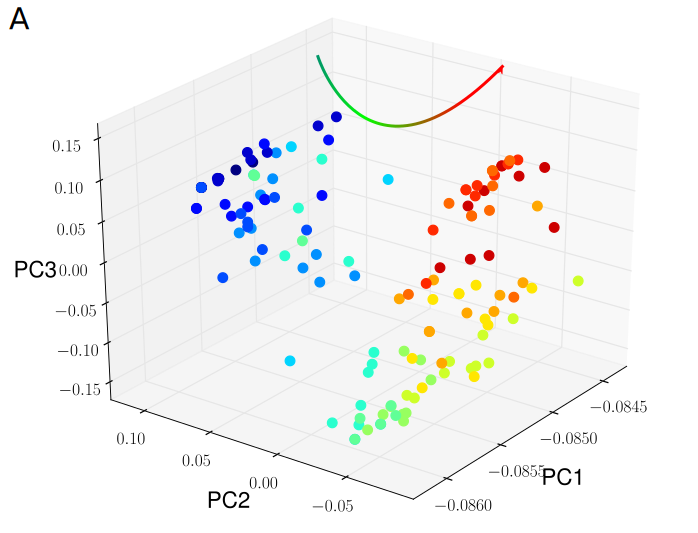
\includegraphics[width=0.35\linewidth]{Shankarappa_PCA_p1}
\includegraphics[width=0.35\linewidth]{Shankarappa_allele_freqs_trajectories_nonsyn_p1}
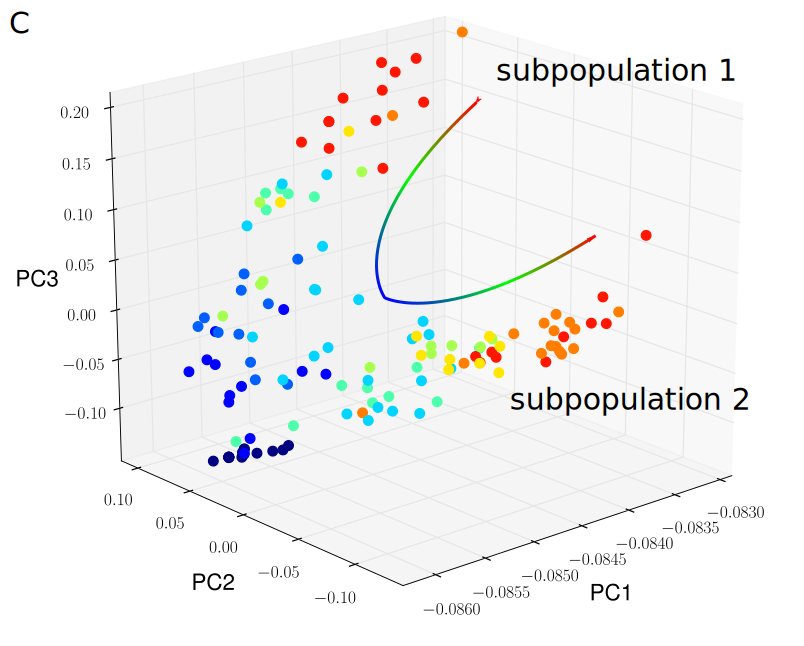
\includegraphics[width=0.35\linewidth]{Shankarappa_PCA_p7}
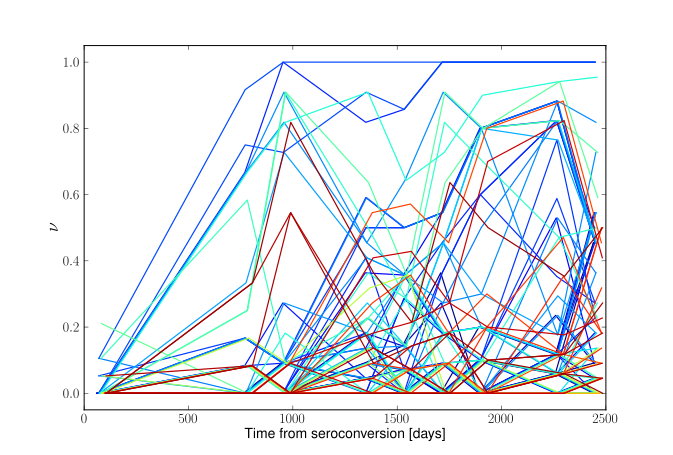
\includegraphics[width=0.35\linewidth]{Shankarappa_allele_freqs_trajectories_nonsyn_p7}
\caption{Structure of viral populations and patient selection.
Panel A) shows a PCA of all sequences from patient p1 (colors indicate time from
seroconversion, from blue to red). Panel B) shows allele frequency trajectories for nonsynonymous
changes in the same patient. Here, the blue to red color map corresponds to the
position of the allele in \env{} from 5' to 3'. Panels C) and D) show analogous
plots for data from patient p7. Samples after day 1000 split into two clusters
in the PCA and no single nucleotide variants (SNVs) that arise after day 1000 fix, presumably because they are restricted
to one subpopulation. All patients like p7 (p4, p7, p8, p9 from ref.~\citealp{shankarappa_consistent_1999} and
ACH19542 and ACH19768 from ref.~\citealp{bunnik_autologous_2008}) were excluded
from our analysis.}
\label{fig:aftp}
\end{center}
\end{figure}

\newpage
% %%%%%%%%%%%%%%%%%%%%%%%%%%%%%%%%%%%%%%%%%%%%%%%%%%%%%%%%%%%%%%%%%%%%%%%%
\section{Synonymous diversity across the HIV genome}
% %%%%%%%%%%%%%%%%%%%%%%%%%%%%%%%%%%%%%%%%%%%%%%%%%%%%%%%%%%%%%%%%%%%%%%%%
\begin{figure}[h]
\begin{center}
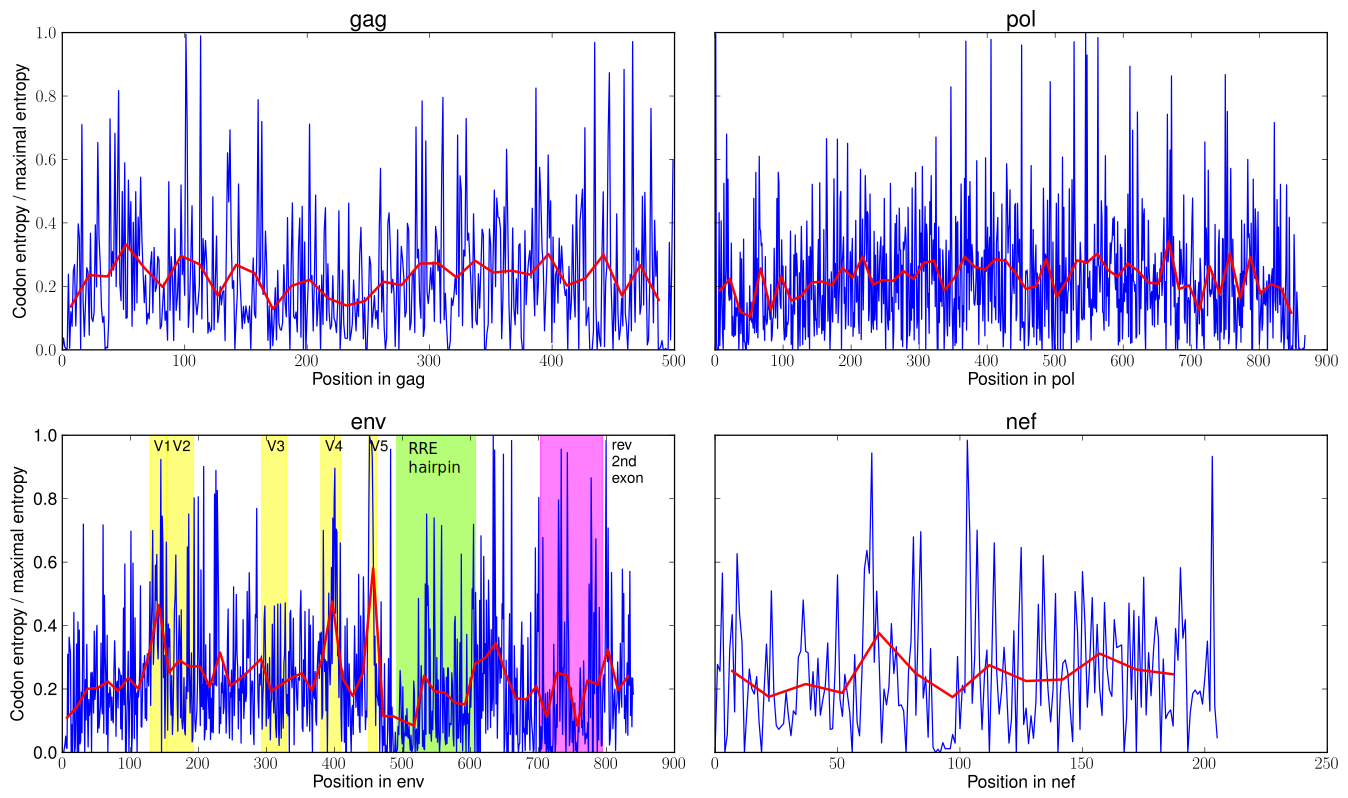
\includegraphics[width=\linewidth]{conservation_codons_genome}
\caption{
Synonymous diversity across the HIV genome, as quantified by the normalized
codon entropy among sequences coding for the consensus amino acid. In most
parts of the genome, synonymous sites show little conservation. The synonymous
diversity peaks at the variable regions in {\it env} and is reduced in regions 
under purifying selection (RRE hairpin, second {\it tat}/{\it rev} exons). The
normalized codon entropy is calculated as follows (see the script
\texttt{codon\_entropy\_synonymous\_subtypeB.py} for the full algorithm): (i)
from a subtype B multiple sequence alignment (MSA) from the LANL website (filtered sequences only, version 2011)~\cite{LANL2012}, we calculate the
consensus amino acid at each position in the HIV genome; (ii) we count how often
each codon coding for the consensus amino acid appears in the MSA; (iii) at each
amino acid position, we divide by the number of sequences in the MSA that had
the consensus amino acid at that position, obtaining {\it codon frequencies}
$\nu_c$; (iv) we calculate the codon entropy from each position as: $S := -
\sum_{c} \nu_c \log \nu_c$, where $c$ runs over codons that code for the
consensus amino acid at this site; (v) we divide by the maximal codon entropy of
that amino acid (e.g. $\log 2$ for twofold degenerate codons). All parts of
{\it env} that are part of a different gene (signaling peptide, second {\it rev}
exon) have been excluded from our main analysis, to avoid contamination by
protein selection in a different reading frame.
Note that all gap-rich columns of the MSA are stripped from this figure, so genes such as {\it env} might appear shorter than they actually
are.
}
\label{fig:syndiv_genome}
\end{center}
\end{figure}
\newpage
% 
% %%%%%%%%%%%%%%%%%%%%%%%%%%%%%%%%%%%%%%%%%%%%%%%%%%%%%%%%%%%%%%%%%%%%%%%%%
% \section{Nonsynonymous changes outside of variable regions are deleterious}
% %%%%%%%%%%%%%%%%%%%%%%%%%%%%%%%%%%%%%%%%%%%%%%%%%%%%%%%%%%%%%%%%%%%%%%%%%
% \begin{figure}[h]
% \begin{center}
% \includegraphics[width=0.8\linewidth]{synmut_conservation_4fold_synnonsyn}
% \caption{Cumulative distribution of synonymous and nonsynonymous diversity in
% {\it gag} in the LANL reference panel (filtered
% sequences only, version 2011)~\cite{LANL2012}. Sites such that the consensus codon
% has three synonymous and six nonsynonymous single mutants were used, and the number of observed mutants
% of a certain type over the number of possible mutants is plotted. Nonsynonymous
% changes are observed less often, {\it ergo} are more conserved, than
% synonymous changes. It can be therefore assumed, as mentioned in the main text,
% that non-escape nonsynonymous changes involve a large fitness cost.}
% \label{fig:synnonsyncons}
% \end{center}
% \end{figure}
% \newpage

%%%%%%%%%%%%%%%%%%%%%%%%%%%%%%%%%%%%%%%%%%%%%%%%%%%%%%%%%%%%%%%%%%%%%%%%%
\section{Time-dependent selection}
%%%%%%%%%%%%%%%%%%%%%%%%%%%%%%%%%%%%%%%%%%%%%%%%%%%%%%%%%%%%%%%%%%%%%%%%%
\begin{figure}[h]
\begin{center}
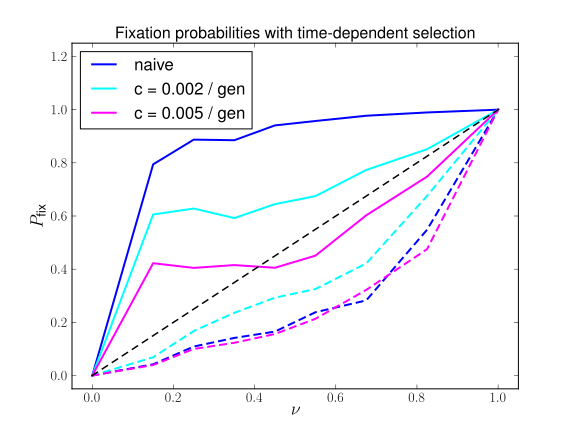
\includegraphics[width=0.6\linewidth]{simulations_gradually_timeselec_deadagain}
\caption{
Time-dependent selection reduces fixation of nonsynonymous SNVs. The figure
compares the fixation probability in the time independent model (na\"ive) to
a model with time dependent selection that mimics  an evolving immune system.
It has been found that virus is typically neutralized by serum from a few months
earlier~\citep{richman_rapid_2003} but not by contemporary serum. We model this
evolving immune system by assuming that escaped variants lose their beneficial
effect with a rate proportional to the frequency of the escaped variant. 
Specifically, the selection effect of the escape mutations is
reset to its fitness cost of $-0.02$ with probability
\[ P_\text{recognized}(t) = c \cdot \nu(t), \] 
per generation, where $c$ is a constant coefficient shown in the legend that
encodes the overall efficiency of the host immune system. With increasing
probability of recognition, the fixation of frequent escape mutants is reduced,
while hitch-hiking of synonymous SNVs is not affected. The precise
shape of $\pfix(\nu)$ depends on the details of the $P_\text{recognized}(t)$, and 
we do not think that the high $\pfix(\nu)$ for $\nu<0.2$ is meaningful.
The other parameters for the shown simulations are
the following: deleterious effect $s_d = 2 \cdot 10^{-3}$, average escape rate $\epsilon
= 0.032$, fraction of deleterious synonymous mutations $\alpha = 0.986$, rate of new epitopes
$k_A=0.0014$ per generation.
}
\label{fig:tds}
\end{center}
\end{figure}

\newpage
%%%%%%%%%%%%%%%%%%%%%%%%%%%%%%%%%%%%%%%%%%%%%%%%%%%%%%%%%%%%%%%%%%%%%%%%%
\section{Within-epitope competition}
%%%%%%%%%%%%%%%%%%%%%%%%%%%%%%%%%%%%%%%%%%%%%%%%%%%%%%%%%%%%%%%%%%%%%%%%%
\begin{figure}[h]
\begin{center}
\includegraphics[width=0.6\linewidth]{simulations_gradually_epitopes}
\caption{
Competition between escape SNVs in the same epitope reduces fixation of
nonsynonymous SNVs. The figure compares the fixation probability of models
with one, three, or six mutually exclusive escape mutations within the
same epitope. Within epitope competition results in reduced fixation
probabilities of nonsynonymous changes, whereas the synonymous changes behave 
similarly in all cases. We assume that escape can happen at $n$ sites out of 3
consecutive codons and vary $n$.
The fitness landscape of each epitope includes negative epistatic terms, so that
the joint presence of more than one escape mutation is not any more beneficial
for the virus than a single mutation. Specifically, each site has two alleles,
$\pm 1$, where $-1$ is the ancestral one and $+1$ the derived one; the fitness
coefficient of a $k$-tuple of sites within the epitope is $f_k = (-1)^{k-1}
2^{1-n}\eta_\epsilon $, where $\eta_\epsilon$ is the escape rate of the epitope
drawn from an exponential distribution with mean $\epsilon$ and 
$n$ is the number of competing escapes in the epitope. 
In this evolutionary scenario, many escape SNVs start to sweep on different backgrounds within the viral population, but eventually
compete and only one of them fixes. The other parameters for the shown simulations are
the following: deleterious effect $s_d = 2 \cdot 10^{-3}$, average escape rate
$\epsilon = 0.032$, fraction of deleterious synonymous mutations $\alpha = 0.986$, rate of new epitopes
$k_A=0.0014$ per generation.
}
\label{fig:wec}
\end{center}
\end{figure}

\newpage
%%%%%%%%%%%%%%%%%%%%%%%%%%%%%%%%%%%%%%%%%%%%%%%%%%%%%%%%%%%%%%%%%%%%%%%%%%
%\section{Simulations with different parameters}
%%%%%%%%%%%%%%%%%%%%%%%%%%%%%%%%%%%%%%%%%%%%%%%%%%%%%%%%%%%%%%%%%%%%%%%%%%
%\begin{figure}[h]
%\begin{center}
%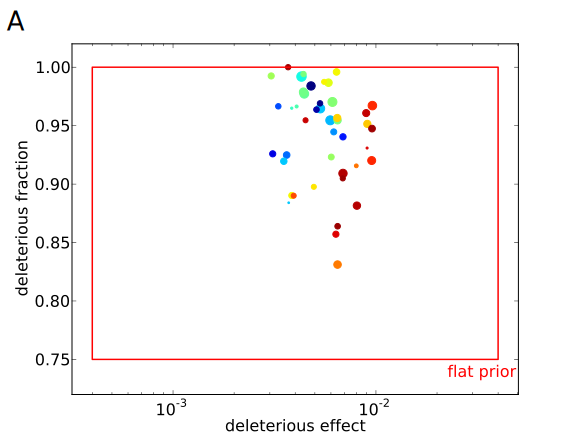
\includegraphics[width=0.4\linewidth]{simulations_syn_gentime_2days.pdf}\\
%\includegraphics[width=0.24\linewidth]{simulations_syn_mu_1e-5.pdf}
%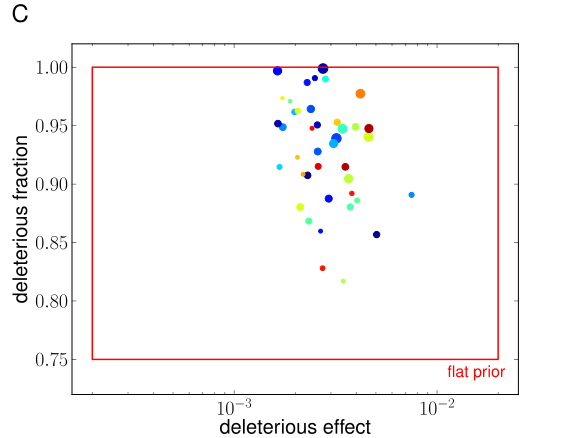
\includegraphics[width=0.24\linewidth]{simulations_syn_latin_suppl.pdf}
%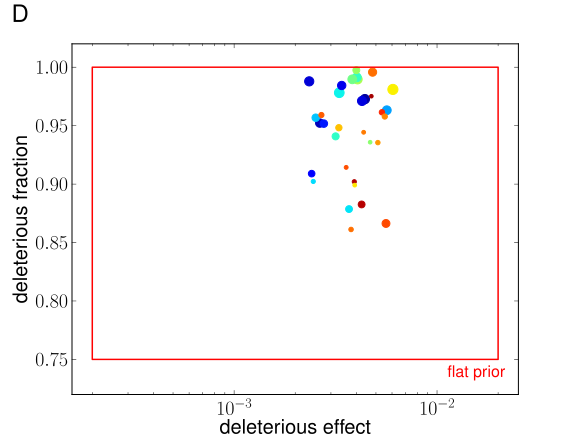
\includegraphics[width=0.24\linewidth]{simulations_syn_mu_3e-5.pdf}
%\includegraphics[width=0.24\linewidth]{simulations_syn_mu_4e-5.pdf}\\
%\includegraphics[width=0.32\linewidth]{simulations_syn_coi_5e-3.pdf}
%\includegraphics[width=0.32\linewidth]{simulations_syn_latin_suppl2.pdf}
%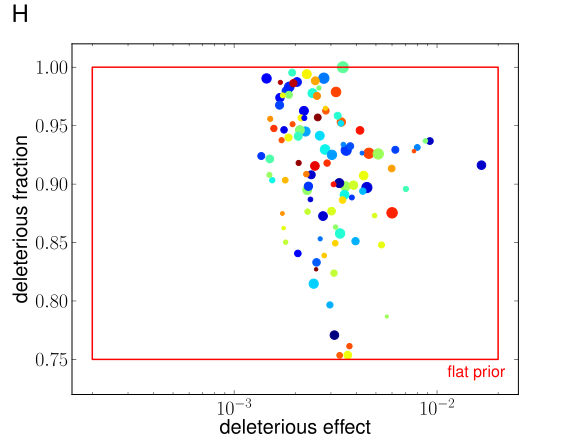
\includegraphics[width=0.32\linewidth]{simulations_syn_coi_2e-2.pdf}
%\caption{
%Results of simulations with alternative parameters.
%\textbf{Panel A)} Like \figurename~4B in the main text, but simulations are performed using a
%generation time of two days. Two selection coefficient of synonymous sites
%doubles in units of 1/generations, hence keeps constants in units of 1/days.
%\textbf{Panels B, C, D, and E)} Effect of mutation rate on the simulation
%results. The mutation rates are respectively $1 \times 10^{-5}$ (B), $2 \times
%10^{-5}$ (C), $3 \times 10^{-5}$ (D), and $4 \times
%10^{-5}$ (E) per generation per site. Increasing the mutation rate tightens the
%requirement that almost all synonymous mutations must be deleterious. This can
%be rationalized as follows: a higher $\mu$ increases the neutral synonymous
%diversity (we have measured this directly in our simulations), hence more and
%more synonymous SNVs that reach high frequency are neutral and the
%effect of deleterious SNVs, although present, becomes too weak to be observed as
%a depression in $P_\text{fix}$. As a consequence, only simulations with almost
%no neutral sites still show a reduced $P_\text{fix}$ and are shown in the
%figures.
%\textbf{Panels F, G, H)} Effect of recombination rate on the simulation results.
%The recombination rates are respectively $0.5 \times 10^{-5}$ (F), $10^{-5}$
%(G), and $2 \times 10^{-5}$ (H) per generation per site. Recombination does not
%change the results qualitatively in terms of fixation probability. Simulations
%with high recombination rates, however, have an excessively high synonymous
%diversity compared to the data (dots at the bottom and right side of panel H).
%More stringent gating around the data solves this issue.
%}
%\label{fig:sims_altparameters}
%\end{center}
%\end{figure}


\newpage
%%%%%%%%%%%%%%%%%%%%%%%%%%%%%%%%%%%%%%%%%%%%%%%%%%%%%%%%%%%%%%%%%%%%%%%%%
\section{Marginal distributions in simulations}
%%%%%%%%%%%%%%%%%%%%%%%%%%%%%%%%%%%%%%%%%%%%%%%%%%%%%%%%%%%%%%%%%%%%%%%%%
\begin{figure}[h]
\begin{center}
\includegraphics[width=0.99\linewidth]{simulations_syn_marginals.pdf}
\caption{
Marginal distributions of parameters in simulations that reproduce the
synonymous fixation probability and diversity seen in the data. The prior on all
parameters are flat lines (see methods). Whereas some parameters do not seem to
affect the fixation of synonymous deleterious SNVs (e.g. the recombination
rate), the effect of deleterious synonymous changes and their abundance are
crucial, as discussed in the main text.
}
\label{fig:sims_altparameters}
\end{center}
\end{figure}


\newpage
%%%%%%%%%%%%%%%%%%%%%%%%%%%%%%%%%%%%%%%%%%%%%%%%%%%%%%%%%%%%%%%%%%%%%%%%%
\section{Divergence and diversity over time in simulations}
%%%%%%%%%%%%%%%%%%%%%%%%%%%%%%%%%%%%%%%%%%%%%%%%%%%%%%%%%%%%%%%%%%%%%%%%%
\begin{figure}[h]
\begin{center}
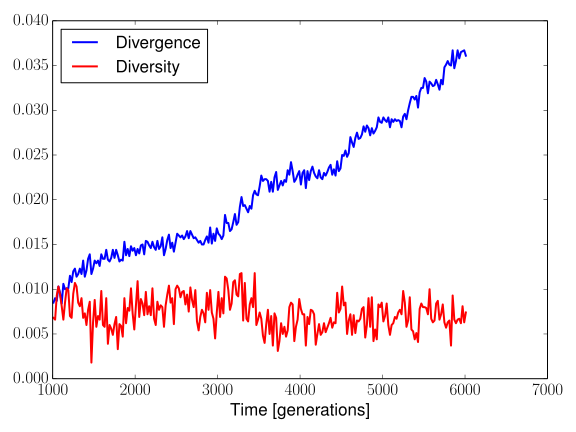
\includegraphics[width=0.6\linewidth]{simulations_diversity_divergence_example.pdf}
\caption{
Diversity and divergence over time in an example simulation with realistic
parameters. Divergence from the founder genotype accumulates linearly. On the
contrary, because of the frequent selective sweeps of escape mutations, diversity saturates
relatively quickly. The population dynamics after that point is in a steady
state.
}
\label{fig:sims_altparameters}
\end{center}
\end{figure}


%%%%%%%%%%%%%%%%%%%%%%%%%%%%%%%%%%%%%%%%%%%%%%%%%%%%%%%%%%%%%%%%%%%%%%%%%
\end{document}
%%%%%%%%%%%%%%%%%%%%%%%%%%%%%%%%%%%%%%%%%%%%%%%%%%%%%%%%%%%%%%%%%%%%%%%%%
